%----------------------------------------------------------------------------------------
%    PACKAGES AND THEMES
%----------------------------------------------------------------------------------------

\documentclass[aspectratio=169,xcolor=dvipsnames,10pt]{beamer}
\usetheme{SimplePlus}

\usepackage{hyperref}
\usepackage{graphicx} % Allows including images
\usepackage{booktabs} % Allows the use of \toprule, \midrule and \bottomrule in tables
\usepackage{amsmath}
\usepackage{ulem} % For underlining

\usepackage{animate}

% \usepackage{better-beamer}
\makeatletter
\renewcommand{\itemize}[1][]{%
  \beamer@ifempty{#1}{}{\def\beamer@defaultospec{#1}}%
  \ifnum \@itemdepth >2\relax\@toodeep\else
    \advance\@itemdepth\@ne
    \beamer@computepref\@itemdepth% sets \beameritemnestingprefix
    \usebeamerfont{itemize/enumerate \beameritemnestingprefix body}%
    \usebeamercolor[fg]{itemize/enumerate \beameritemnestingprefix body}%
    \usebeamertemplate{itemize/enumerate \beameritemnestingprefix body begin}%
    \list
      {\usebeamertemplate{itemize \beameritemnestingprefix item}}
      {\def\makelabel##1{%
          {%
            \hss\llap{{%
                \usebeamerfont*{itemize \beameritemnestingprefix item}%
                \usebeamercolor[fg]{itemize \beameritemnestingprefix item}##1}}%
          }%
        }%
      }
  \fi%
  \setlength\itemsep{\fill}
    \ifnum \@itemdepth >1
        \vfill
    \fi%  
  \beamer@cramped%
  \raggedright%
  \beamer@firstlineitemizeunskip%
}

\def\enditemize{\ifhmode\unskip\fi\endlist%
  \usebeamertemplate{itemize/enumerate \beameritemnestingprefix body end}
  \ifnum \@itemdepth >1
        \vfil
  \fi%  
  }
\makeatother
%----------------------------------------------------------------------------------------
%    TITLE PAGE
%----------------------------------------------------------------------------------------
\title{Cultural Evolution of Human Beauty Standards}
\subtitle{Example of Fashion Modeling}

\author{ \hspace{0.1em}\underline{Louis Boucherie}, Sagar Kumar, Katharina Ledebur, August Lohse, Karolina Sliwa}

% \institute
% {
% \hspace{-0.25em}DTU Compute, Technical University of Denmark \\
% Center for Social Data Science, University of Copenhagen  % Your institution for the title page
% }
% \date{\today} % Date, can be changed to a custom date

%----------------------------------------------------------------------------------------
%    PRESENTATION SLIDES
%----------------------------------------------------------------------------------------

\begin{document}

\begin{frame}
    % Print the title page as the first slide
    \titlepage
\end{frame}

% \begin{frame}{Overview}
%     \tableofcontents
% \end{frame}

%------------------------------------------------
\section{Introduction \& Motivation}
%------------------------------------------------

\begin{frame}{Beauty Standards as Cultural Evolution}
    \begin{itemize}
        \item \textbf{Beauty standards evolution} represents a fundamental cultural process
        \pause \item Understanding how beauty standards and representational norms evolve over time constitutes a central question in cultural and social sciences
        \pause \item  \textbf{Fashion modeling} occupies a distinctive position in contemporary culture as both mirror and molder of beauty standards
        \pause\item Unlike other forms of media representation, fashion runways operate as highly visible, globally distributed platforms
    \end{itemize}
    
    \pause \begin{exampleblock}{Research Question}
        How have beauty standards in fashion modeling evolved over the past two decades, and what does this reveal about broader cultural shifts in human representation?
    \end{exampleblock}
\end{frame}

% \begin{frame}{Research Questions}
%     \begin{enumerate}
%         \pause \item \textbf{How has diversity in fashion modeling evolved} across body measurements, visual traits, and nationality from 2000 to the present?
        
%         \pause \item \textbf{To what extent do observed changes reflect genuine broadening} of beauty standards versus the inclusion of statistical outliers?
        
%        \pause \item \textbf{How do patterns of diversity evolution differ between male and female models}, revealing potential gender-specific beauty standard transformations?
%     \end{enumerate}
    
%     % \vspace{1em}
%     % \begin{alertblock}{Approach}
%     %     Comprehensive quantitative analysis using entropy measures, distribution analysis, and traditional statistical methods
%     % \end{alertblock}
% \end{frame}

% %------------------------------------------------
% \section{Background \& Literature}
% %------------------------------------------------

% \begin{frame}{Academic Diversity Gaps in Fashion}
%     \begin{columns}[c]
%         \column{.5\textwidth}
%         \textbf{Six Major Diversity Categories:}
%         \begin{enumerate}
%             \item Social class
%             \item Body image  
%             \item Race and ethnicity
%             \item Age
%             \item Limited abilities
%             \item Sex and gender
%         \end{enumerate}
        
%         \column{.5\textwidth}
%         \begin{block}{Quantitative Evidence}
%             Marginalized racial and ethnic groups comprise only \textbf{22\%} of high fashion contributors despite representing \textbf{39\%} of the U.S. population
%         \end{block}
        
%         \begin{alertblock}{Health Implications}
%             WHO study: \textbf{66\%} of professional fashion models were underweight, with \textbf{25\%} having BMI below 17.5
%         \end{alertblock}
%     \end{columns}
% \end{frame}

%------------------------------------------------
\section{Methodology}
%------------------------------------------------

\begin{frame}{Data Description}
    \begin{columns}
        \column{0.3\textwidth} % Adjust width as needed
            \begin{figure}
                \foreach \n in {0,...,11} {
                \only<\n>{\includegraphics[width=\textwidth]{figures/ganni/ganni_\n.png}}
                    }
                %\animategraphics[loop,width=\textwidth]{1}{figures/ganni/ganni_}{0}{10}
            \end{figure}
        \pause
        \pause
        \column{0.6\textwidth} % Adjust width as needed
            \vspace{0.6em}
            \begin{itemize}
                \setlength{\itemsep}{0.6em}
                \pause \item 953 000 runway images (2000-present)
                % \vspace{0.6em}
                \begin{itemize}
                    \setlength{\itemsep}{0.3em}
                    \pause \item[] Brand
                    \pause \item[] Collection (year, season)
                \end{itemize}
                \pause \item 250 000 with model annotations
                \pause \item 15 000 model profiles
                % \vspace{0.6em}
                \begin{itemize}
                    \setlength{\itemsep}{0.3em}
                    \pause \item[] Body measurements (height, bust, waist, hips)
                    \pause \item[] Visual traits (hair, eye color)
                    \pause \item[] Nationality
                \end{itemize}
            \end{itemize}
    \end{columns}
\end{frame}



%------------------------------------------------
\section{Body Measurements Evolution}
%------------------------------------------------

\begin{frame}{Body Measurements: Evolution}
    \begin{columns}
        \column{0.7\textwidth}
            \begin{figure}
                    \begin{center}
                    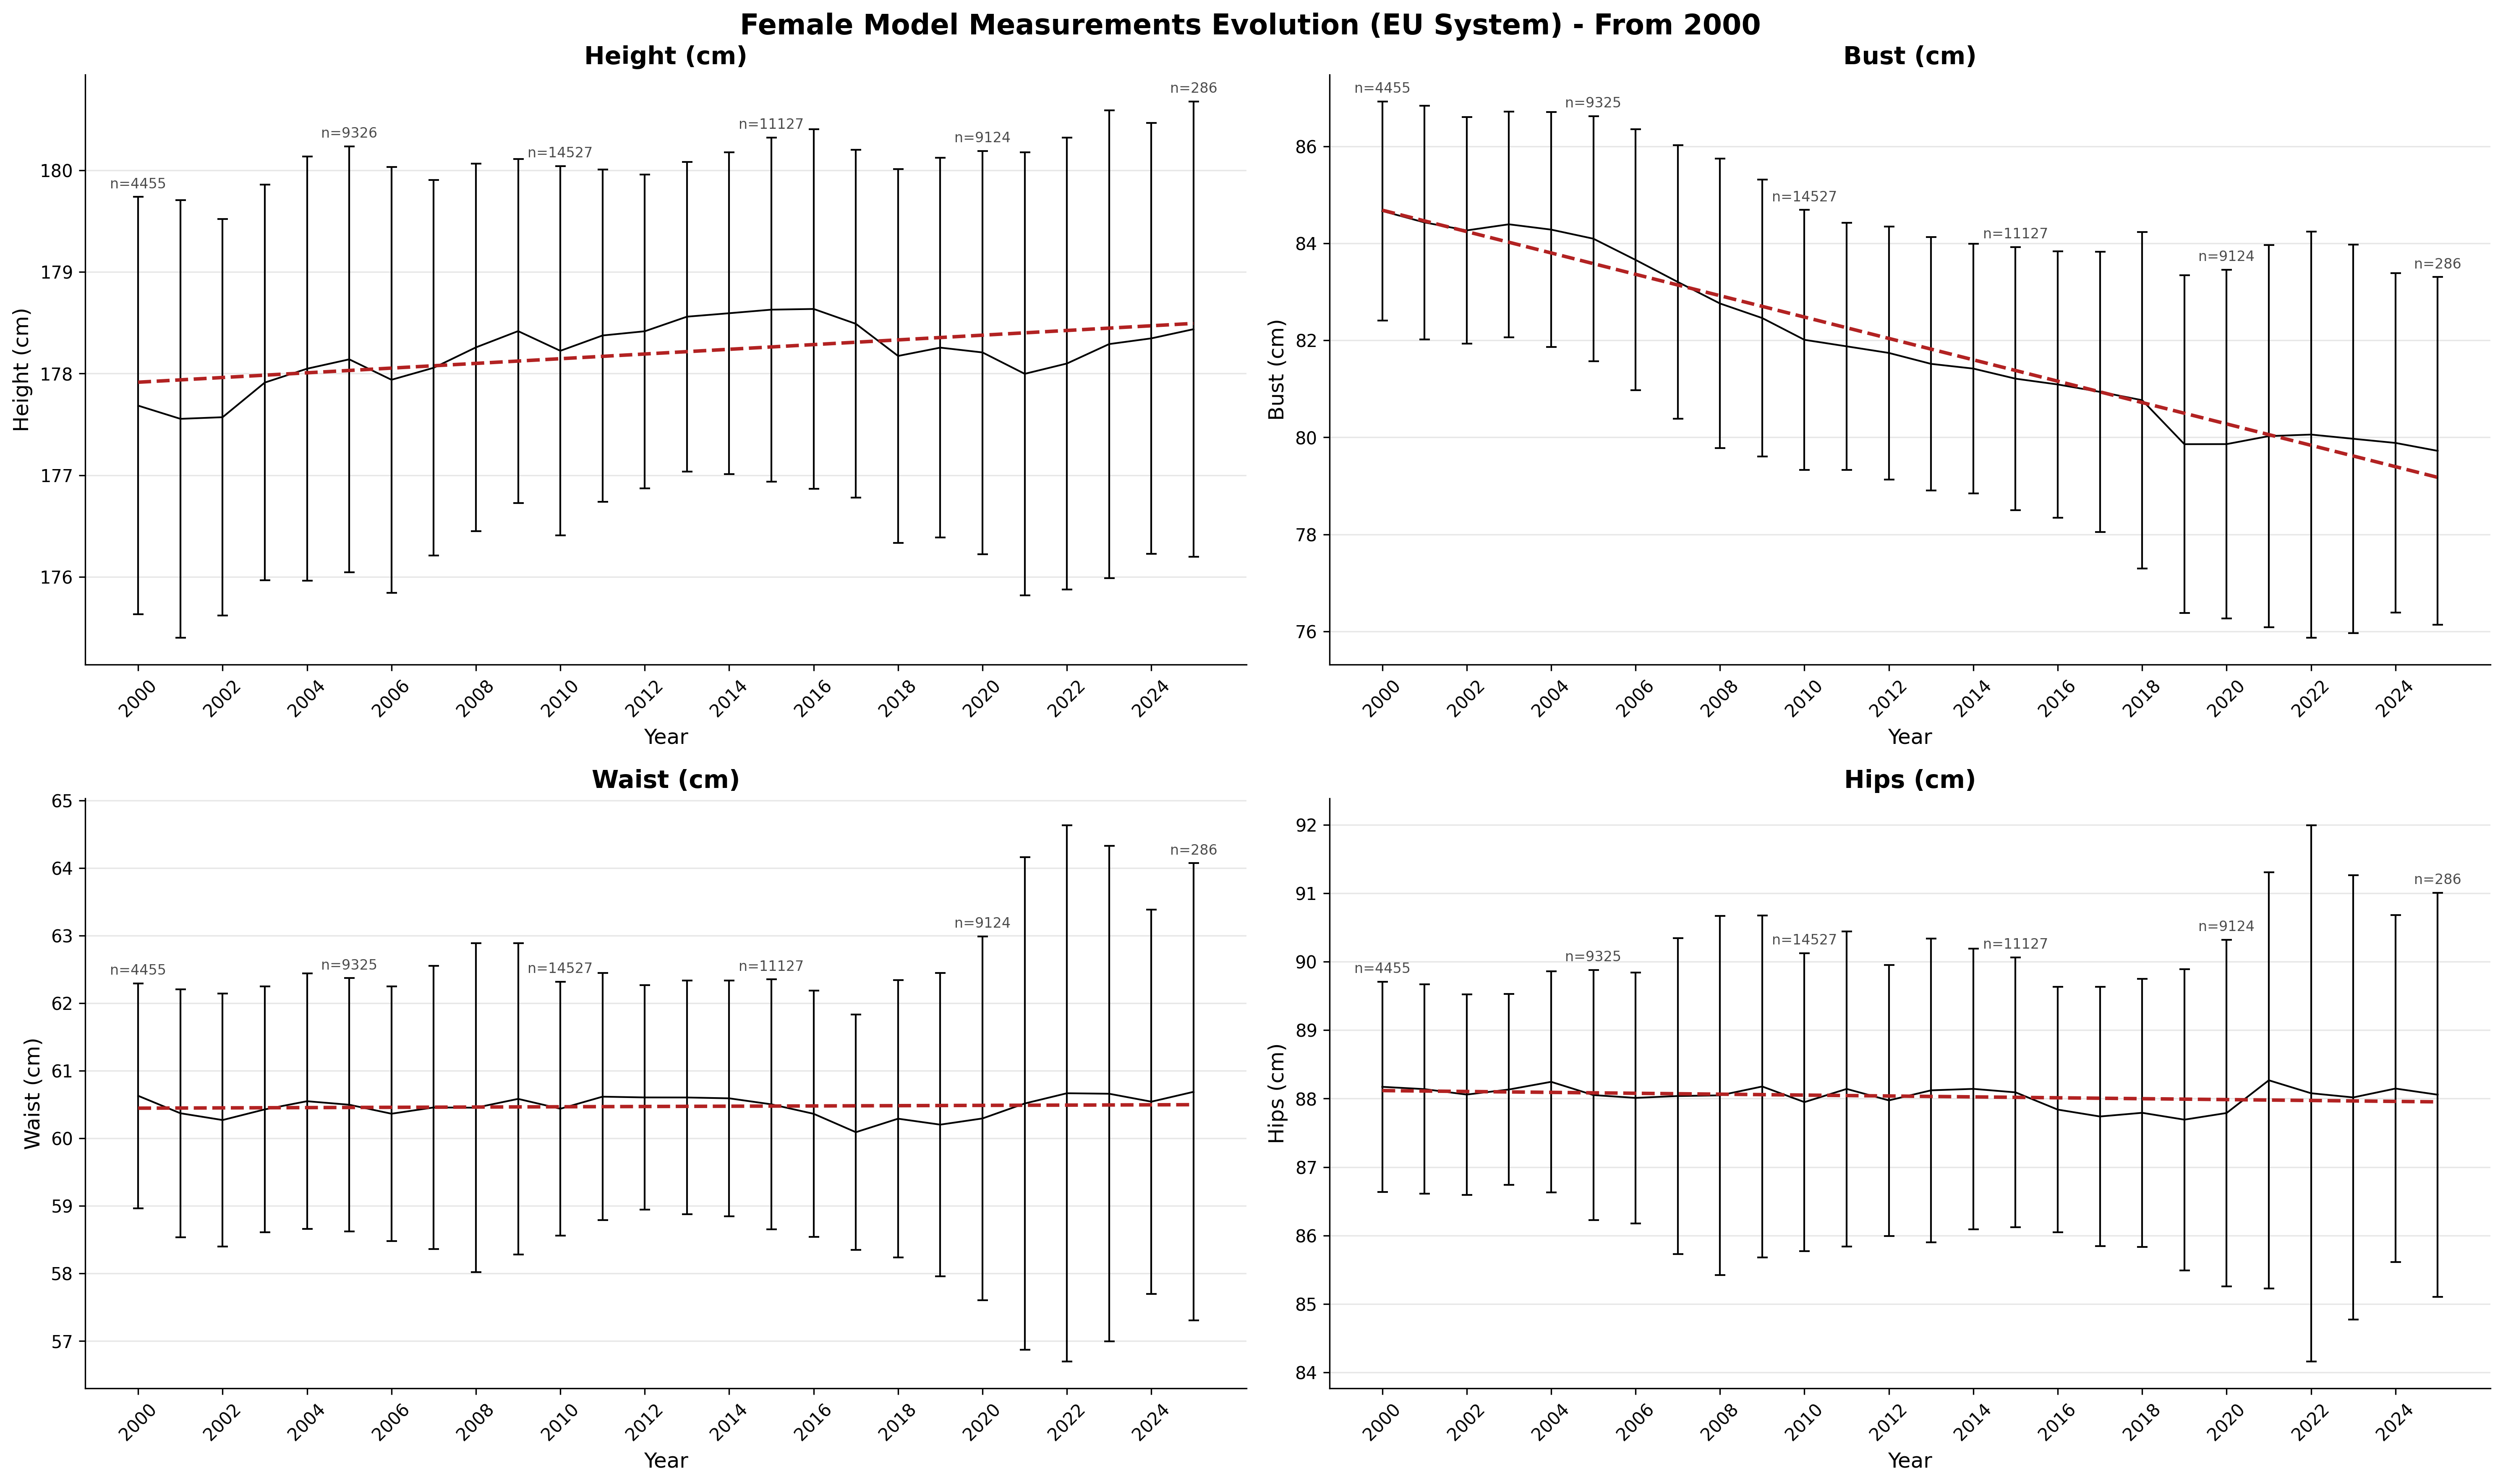
\includegraphics[width=\textwidth]{figures/evolution_female_eu_from_2000.png}
                    \end{center}
                \end{figure}

        \column{0.3\textwidth}
            \raggedright
            \begin{itemize}
                \setlength{\itemsep}{0.6em}
                \pause \item Height: slight increase
                \item Bust: decrease
                \item Waist \& Hips: stable
            \pause
            \vspace{1.2em}
            \item[] \begin{block}{}\textbf{Standard deviations increase across all measurements}
            \end{block}
            \end{itemize}
        \end{columns}
\end{frame}




\begin{frame}{Standard Deviation Trends: Increasing Diversity}
    \begin{figure}
        \begin{center}
        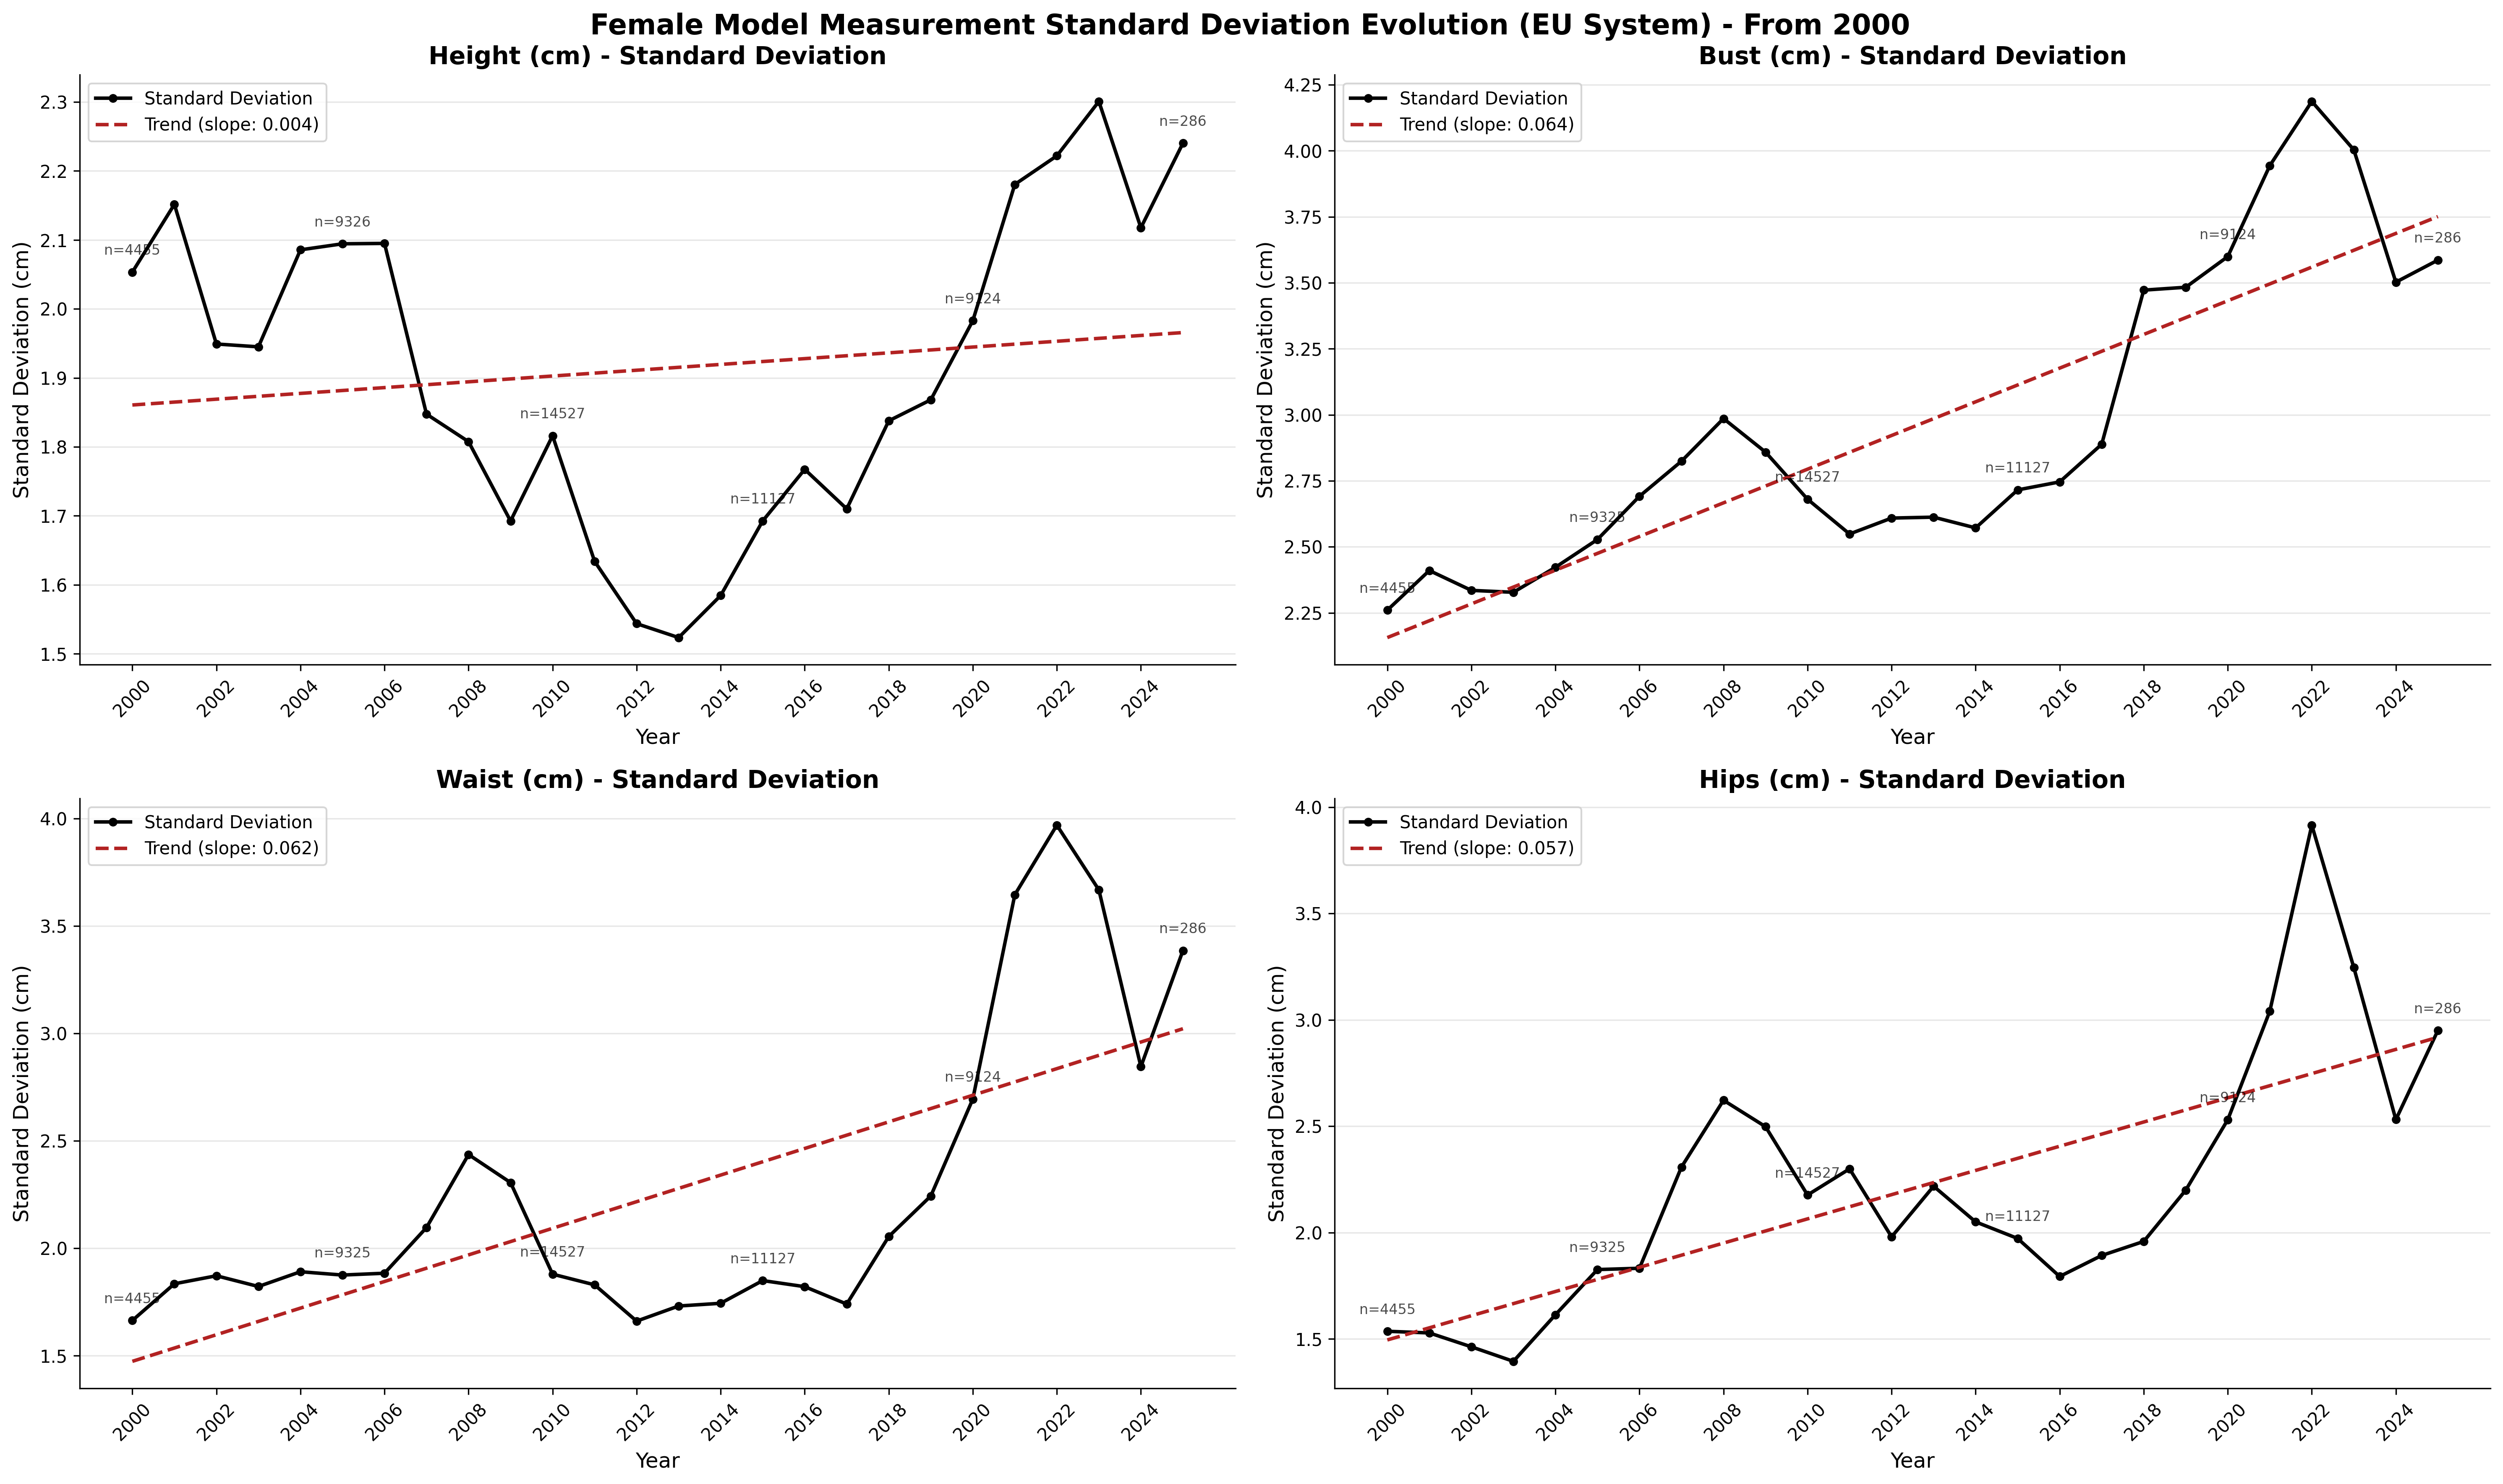
\includegraphics[width=0.65\textwidth]{figures/std_evolution_female_eu_from_2000.png}
        \end{center}
    \end{figure}
    \pause
    \begin{block}\small{The std increase across all measurements indicates broader acceptance of body type variation}
    \end{block}
\end{frame}



%------------------------------------------------
\section{Visual Diversity}
%------------------------------------------------

\begin{frame}{Hair \& Eye Color Evolution}
    \begin{figure}
        \centering
        %\includegraphics[width=0.9\textwidth]{figures/hair_eye_color_by_female.png}
        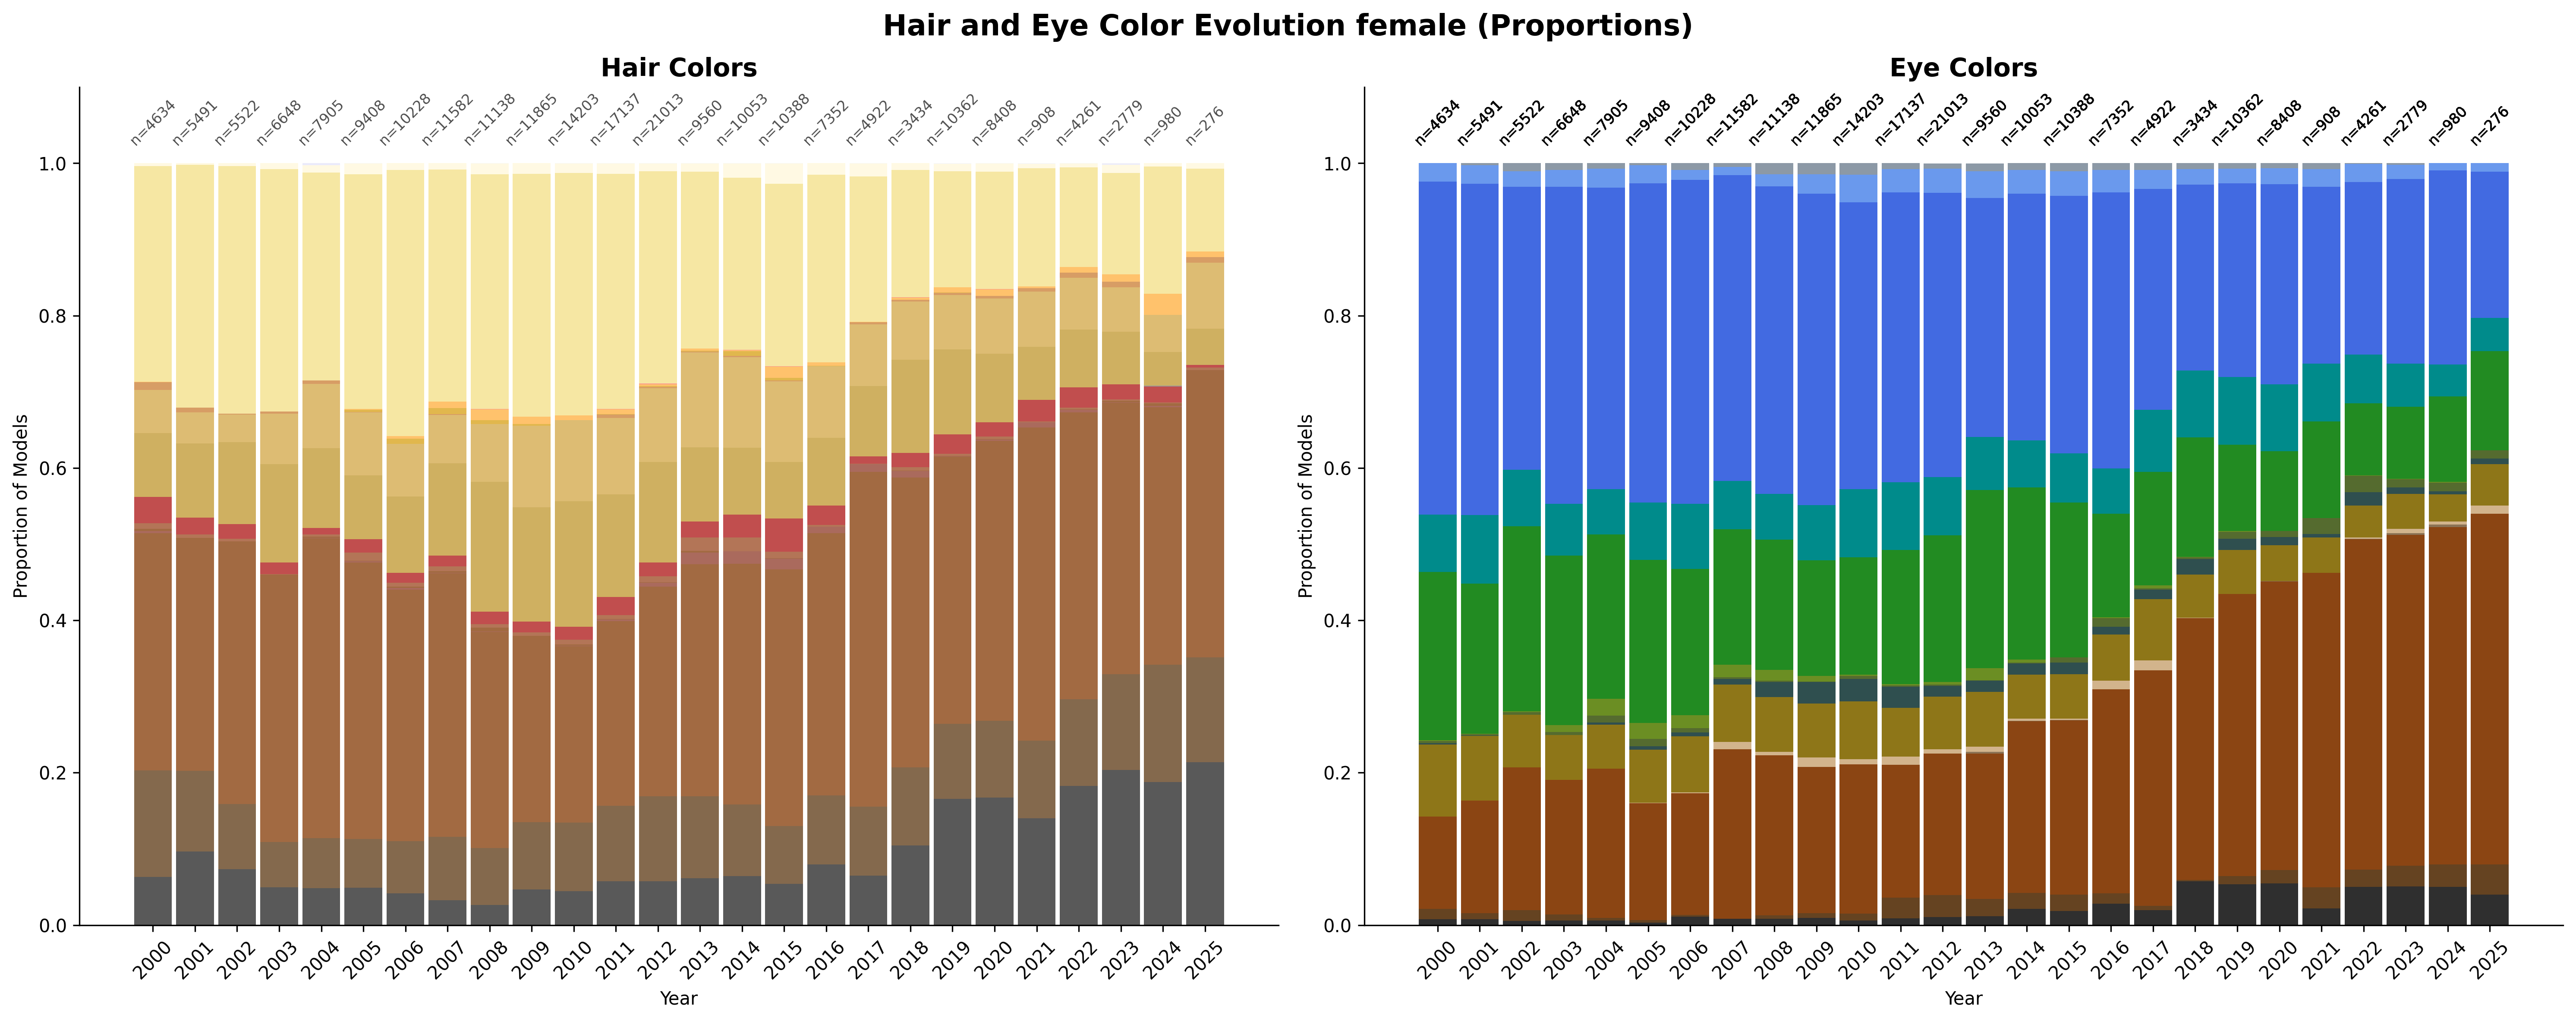
\includegraphics[width=0.9\textwidth]{figures/hair_eye_color_female.png}
    \end{figure}
    
    \begin{columns}[c]
        \column{.5\textwidth}
        \textbf{Hair color trends:}
        \begin{itemize}
            \item Lighter colors (blonde) less dominant
            \item Shift toward darker tones
        \end{itemize}
        
        \column{.5\textwidth}
        \textbf{Eyes color trends:}
        \begin{itemize}
            \item Lighter colors (blue) less dominant
            \item Similar shif than in hair color
        \end{itemize}
    \end{columns}
\end{frame}



%------------------------------------------------
\section{Nationality Diversity}
%------------------------------------------------


\begin{frame}{Global Representation: Entropy Analysis}
    \begin{columns}[c]
        \column{.5\textwidth}
        \begin{figure}
            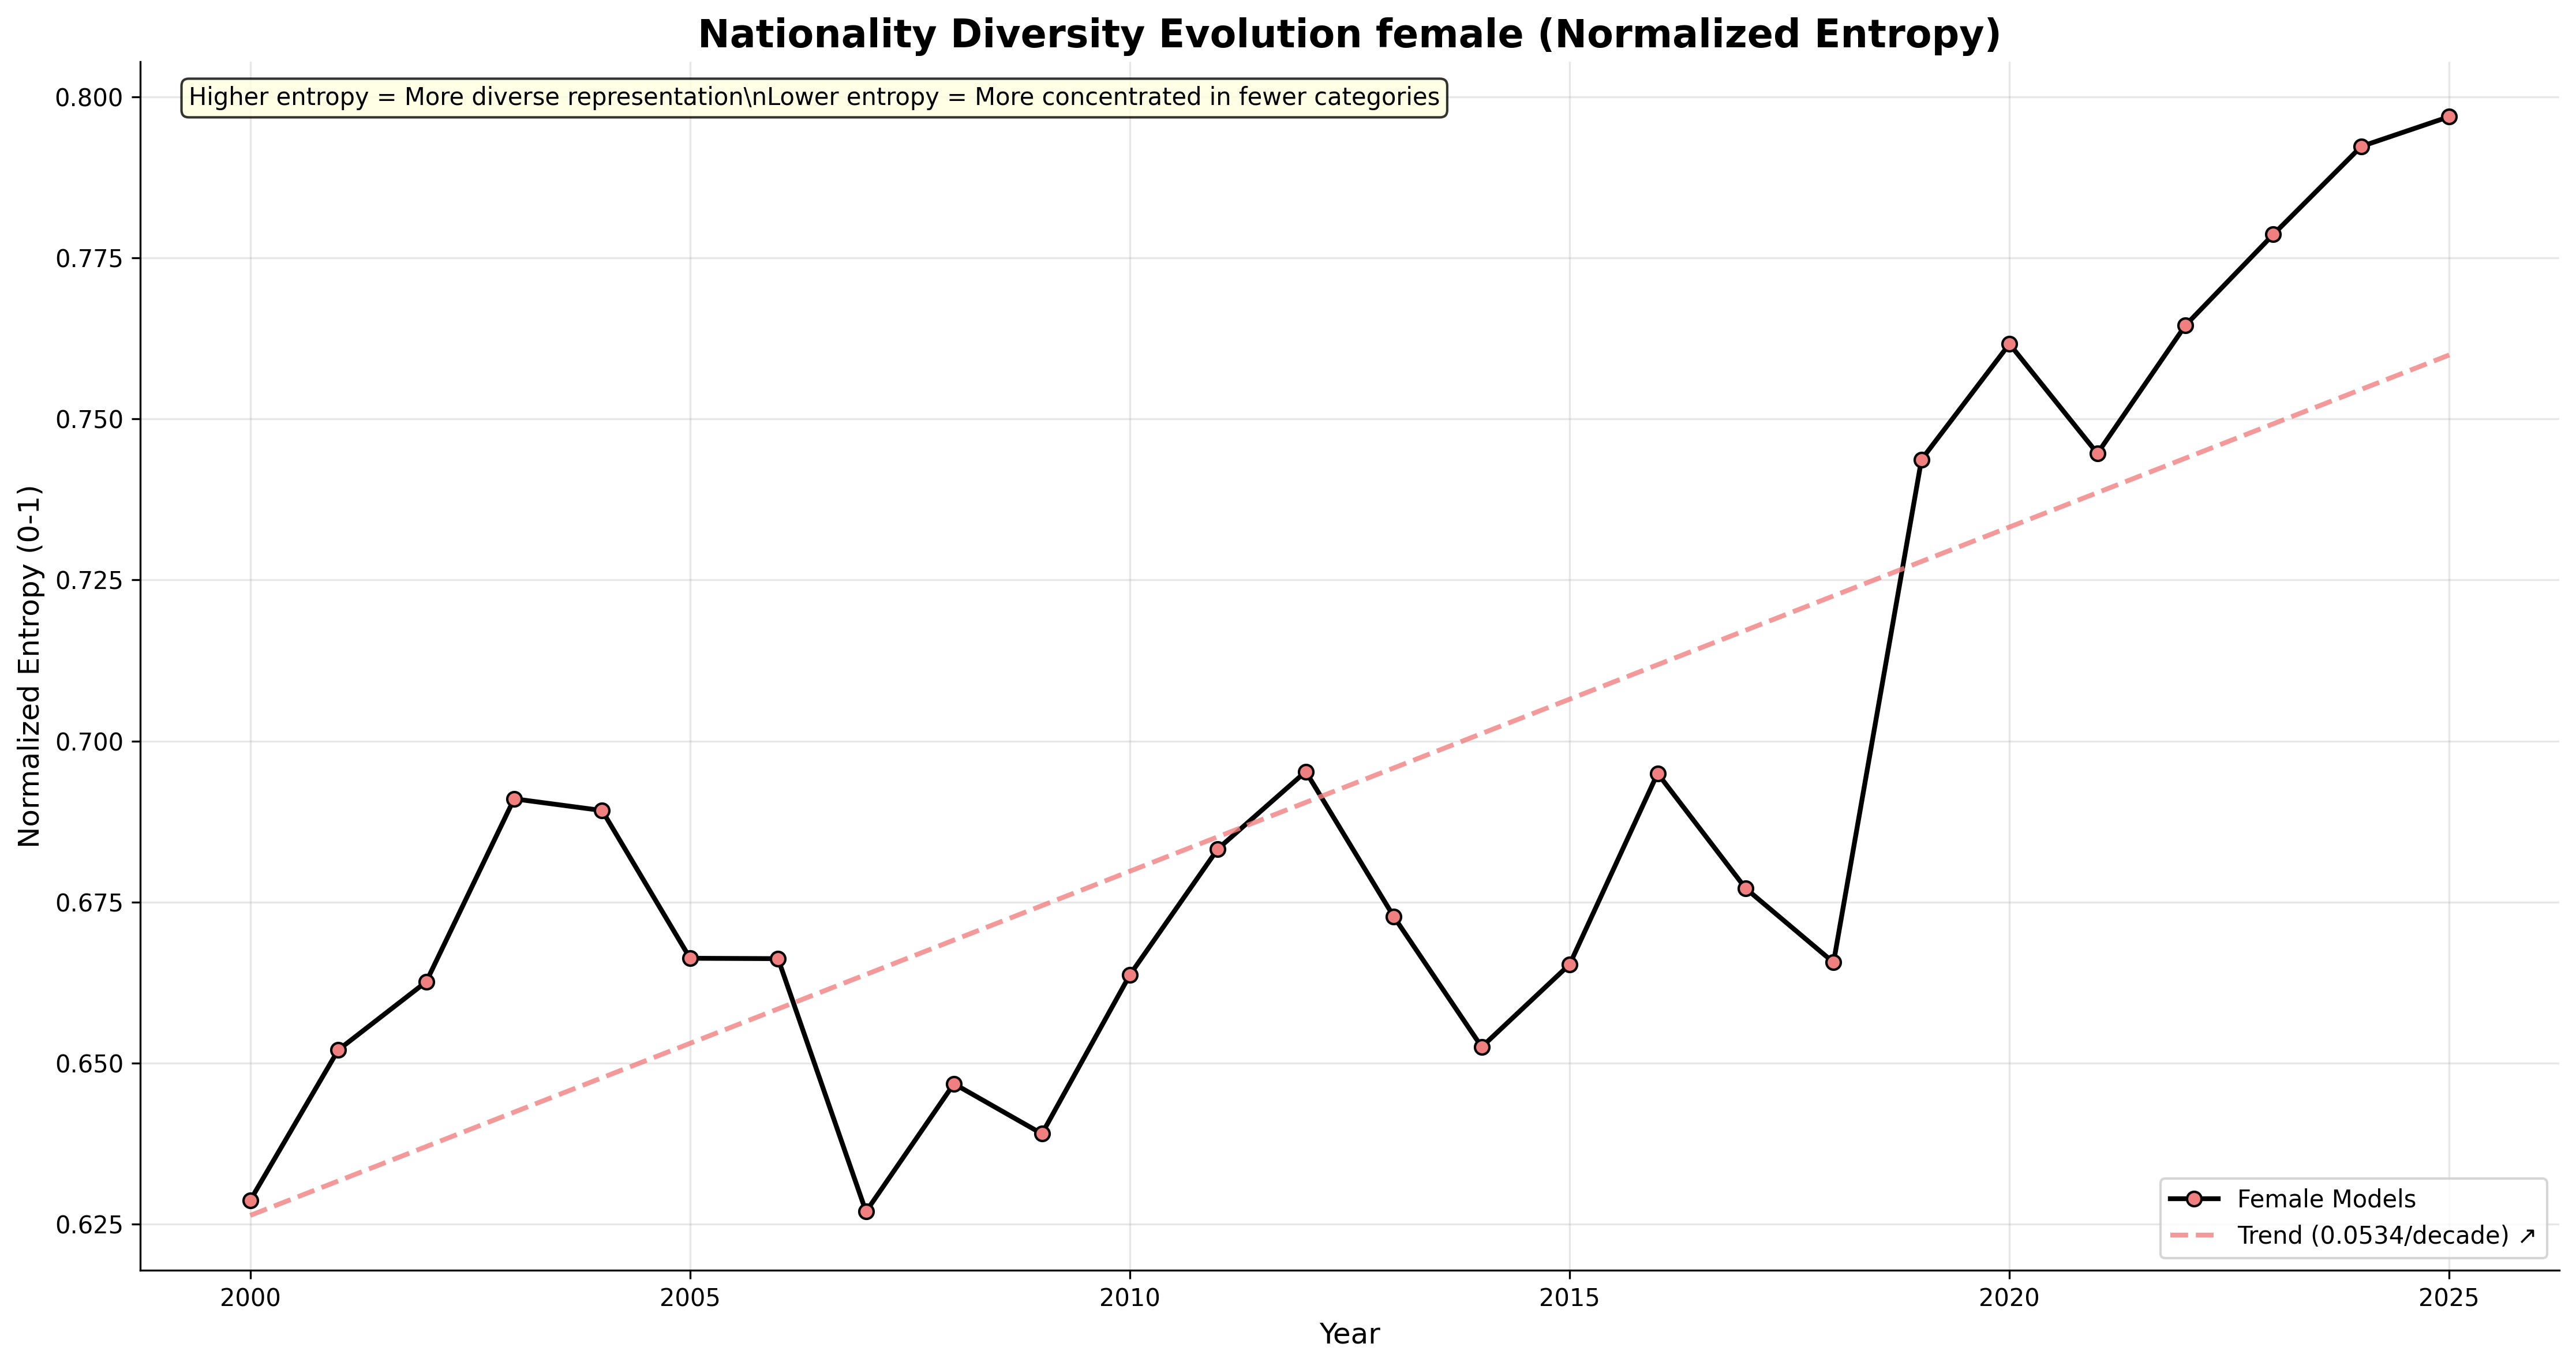
\includegraphics[width=\textwidth]{figures/nationality_entropy_evolution_female.png}
            %\includegraphics[width=\textwidth]{figures/nationality_entropy_evolution_by_female.png}
        \end{figure}
        
        \column{.5\textwidth}
        \textbf{Entropy Growth Rates:}
        \begin{itemize}
            \item \textbf{Female models:} +0.155 bits/decade
            \item Models are more globally representative
        \end{itemize}
        
    \end{columns}
\end{frame}

\begin{frame}{Regional Breakdown}
    \begin{figure}
        \centering
        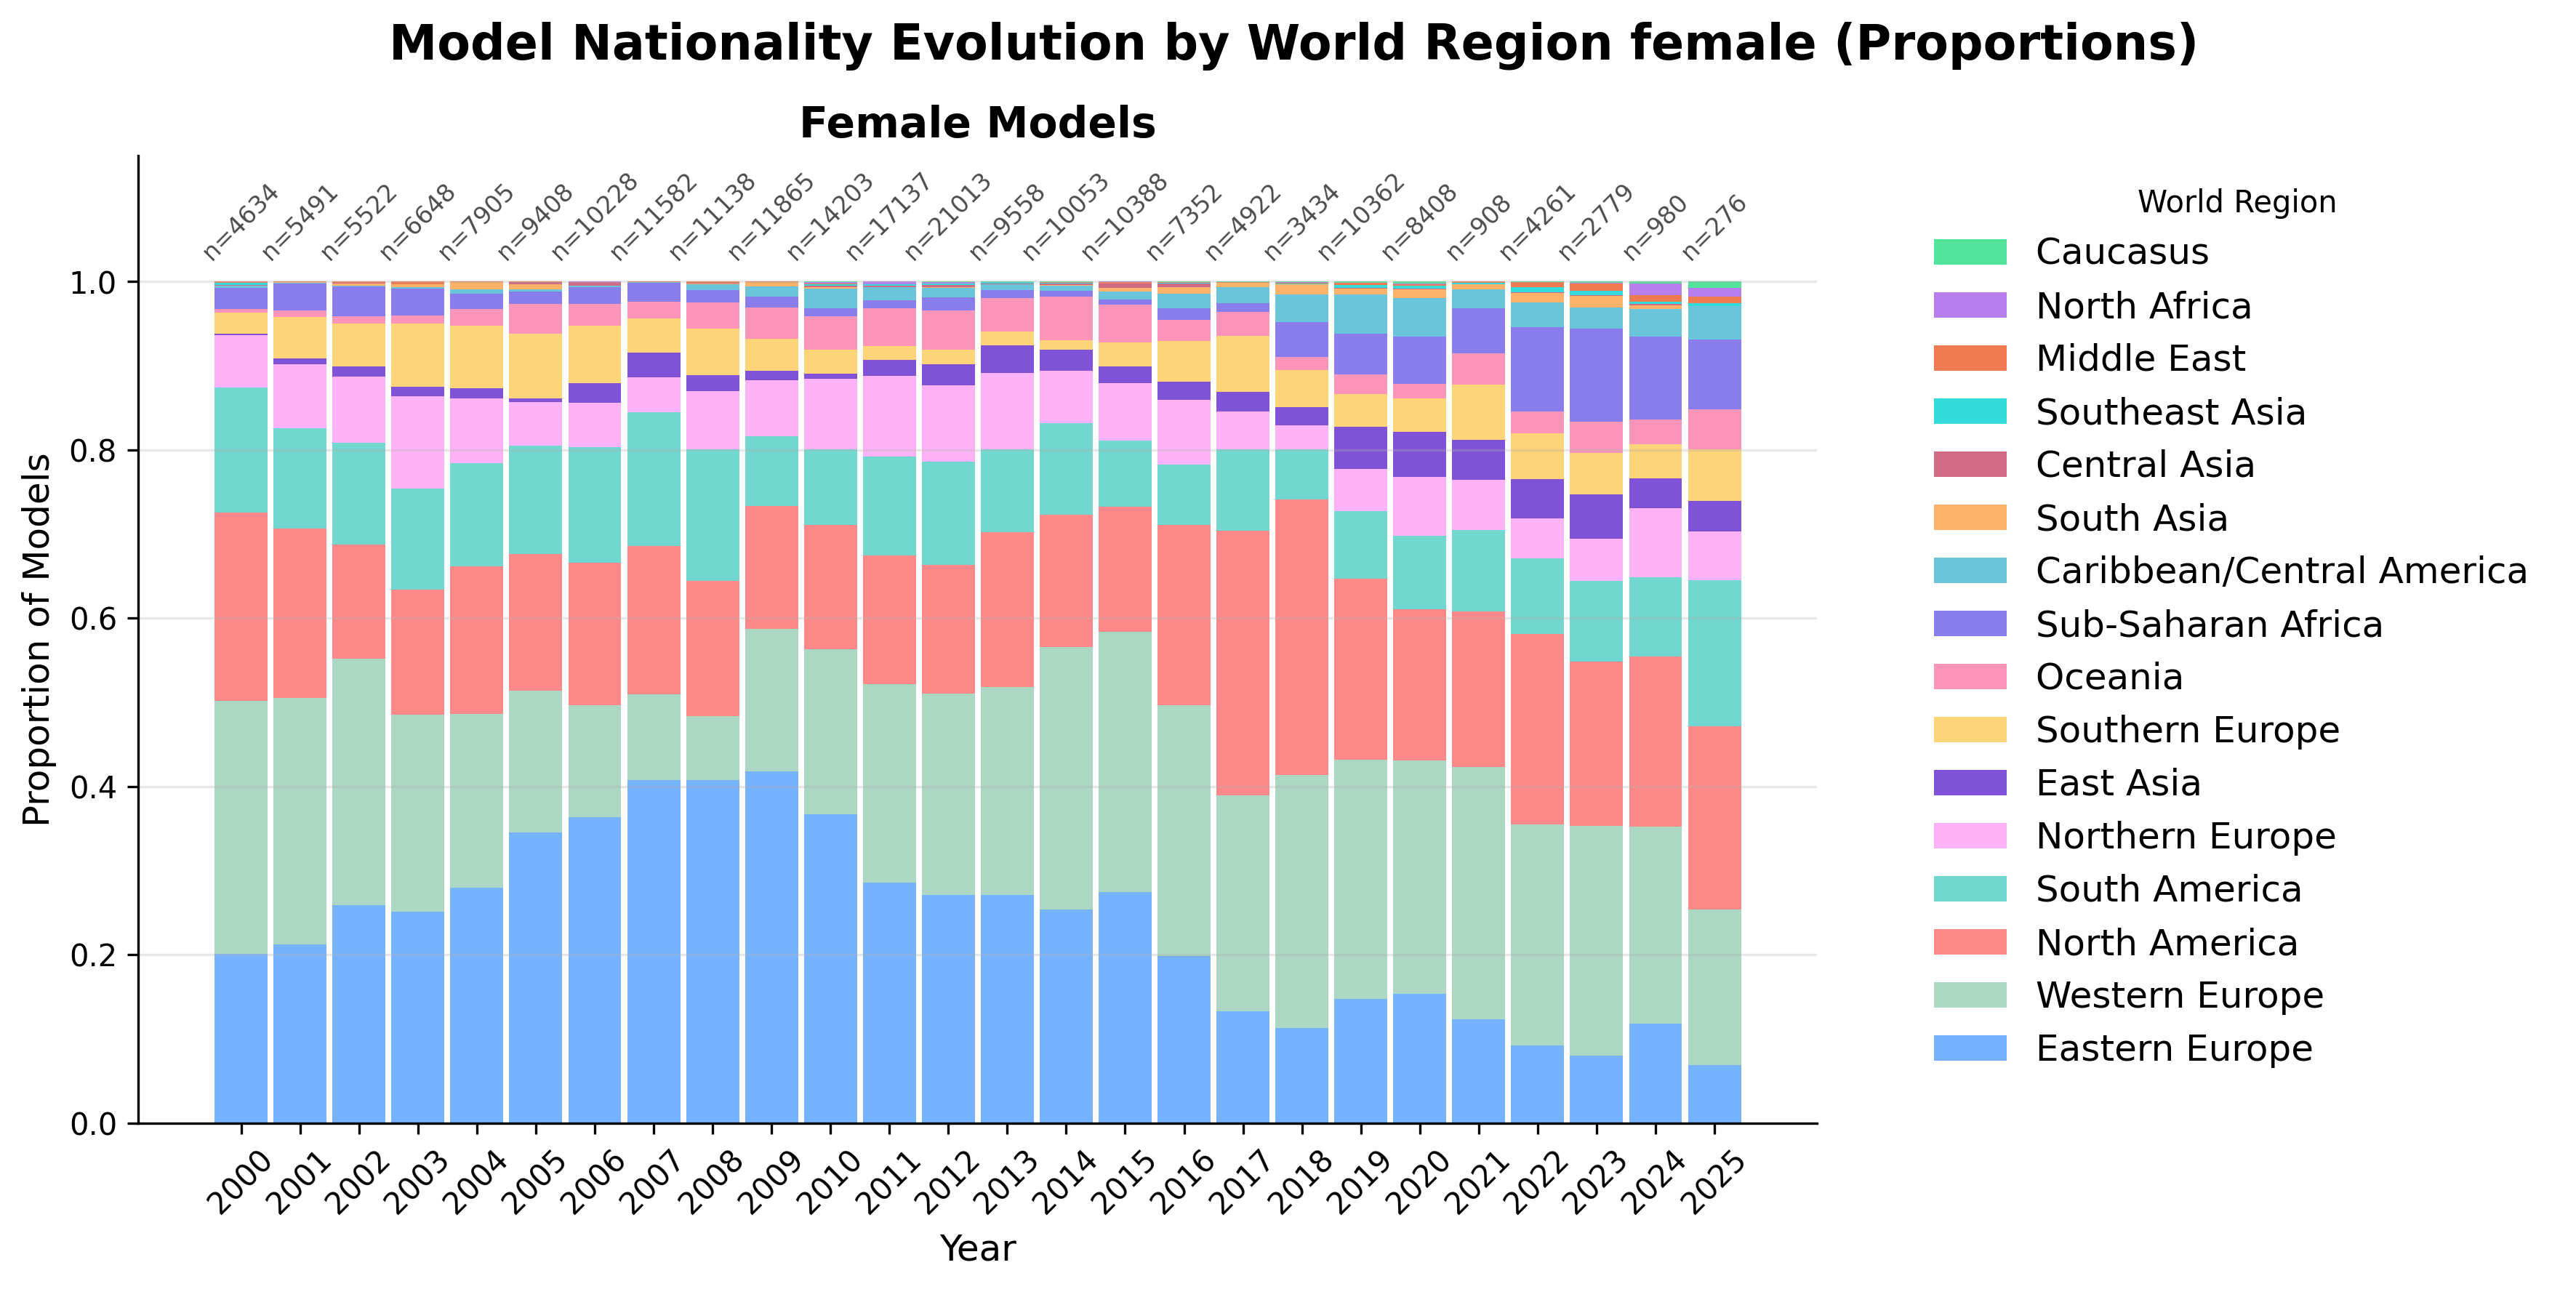
\includegraphics[width=0.85\textwidth]{figures/nationality_evolution_by_region_female.png}
    \end{figure}
    \vspace{-1.5em}
    \begin{block}{}
    Regional breakdown shows increasing representation from Africa, Asia, and South America
    \end{block}
\end{frame}


\begin{frame}{Skin Color Diversity: Individual Typology Angle}
    \begin{figure}
        \centering
        %\includegraphics[width=0.8\textwidth]{figures
    \end{figure}
 ALSO increasing
\end{frame}


\begin{frame}{Diversity Summary} %increase for body measurements, hair/eye color, nationality, skin color
    \begin{itemize}
        \setlength{\itemsep}{0.6em}
        \pause \item Body measurements show increasing variation
        \pause \item Hair and eye colors show increasing diversity, with darker tones rising
        \pause \item Nationality entropy increases, indicating broader global representation
        \pause \item Skin color diversity also increasing
    \end{itemize}
    \pause
    \begin{block}{Key Finding}
        Overall, fashion modeling reflects a trend toward greater diversity in beauty standards.
    \end{block}
\end{frame}


        

%------------------------------------------------
\section{Outliers}
%------------------------------------------------
%transition frame, question in big in the center
\begin{frame}
    \Large{
        \begin{center}
            \textbf{What drives diversity?} \\
            \vspace{1em}
            Is the shape of the distribution changing?\\
            \vspace{1em}
            Or is it just a few outliers?

        \end{center}
    }
\end{frame}

\begin{frame}{Distribution Shape: Skewness}
    \begin{columns}
        \column{0.7\textwidth}
            \begin{figure}
                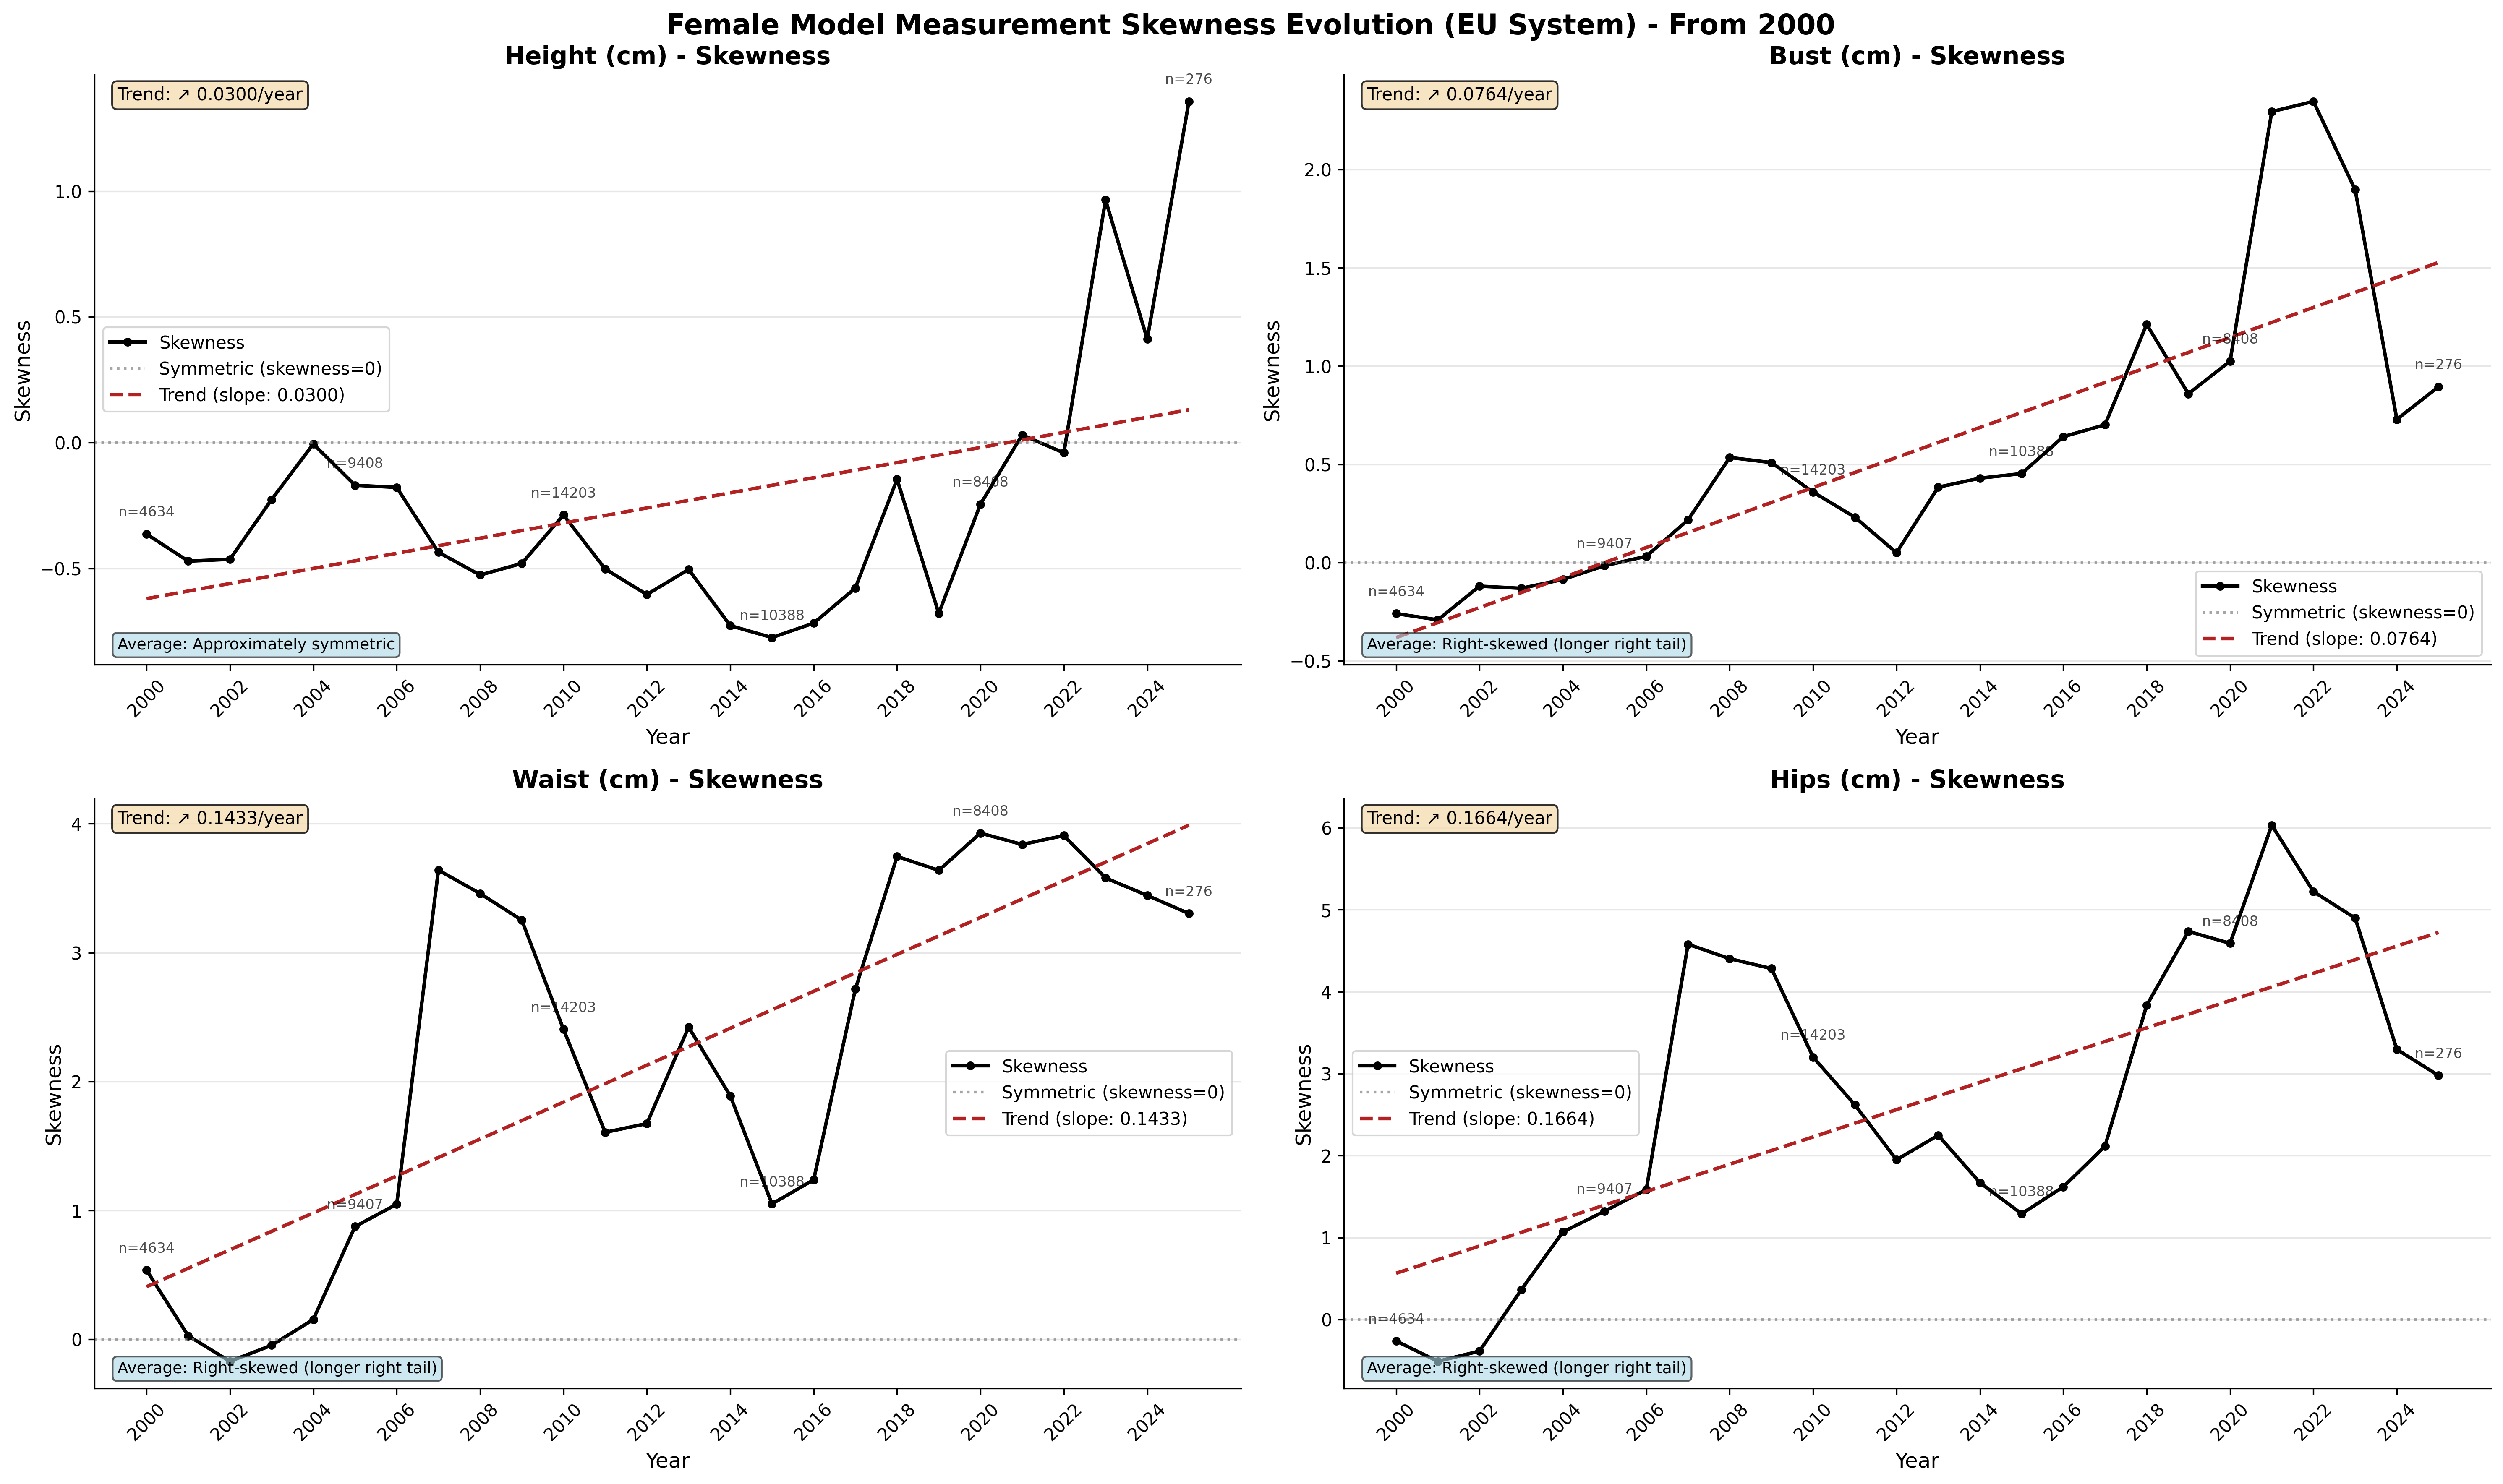
\includegraphics[width=\textwidth]{figures/skewness_evolution_female_eu_from_2000.png}
            \end{figure}
        \column{0.3\textwidth}
        %Skewness shows a shift toward higher values, indicating a trend toward greater acceptance of plus-size models.
        \textbf{Skewness:} 
            \begin{itemize}
                \setlength{\itemsep}{0.6em}
                \pause \item Positive skewness indicates a long tail of larger measurements
                \pause \item Increasing skewness suggests growing acceptance of larger body types
            \end{itemize}
      
    \end{columns}
\end{frame}

\begin{frame}{Distribution Shape: Kurtosis}

    \begin{columns}
    \column{0.3\textwidth}
            %Skewness shows a shift toward higher values, indicating a trend toward greater acceptance of plus-size models.
            \textbf{Kurtosis:} 
                \begin{itemize}
                    \setlength{\itemsep}{0.6em}
                    \item Positive kurtosis indicates a distribution with heavier tails
                    \item Increasing kurtosis suggests more extreme values (outliers) in body measurements
                \end{itemize}
            \column{0.7\textwidth}
                \begin{figure}
                    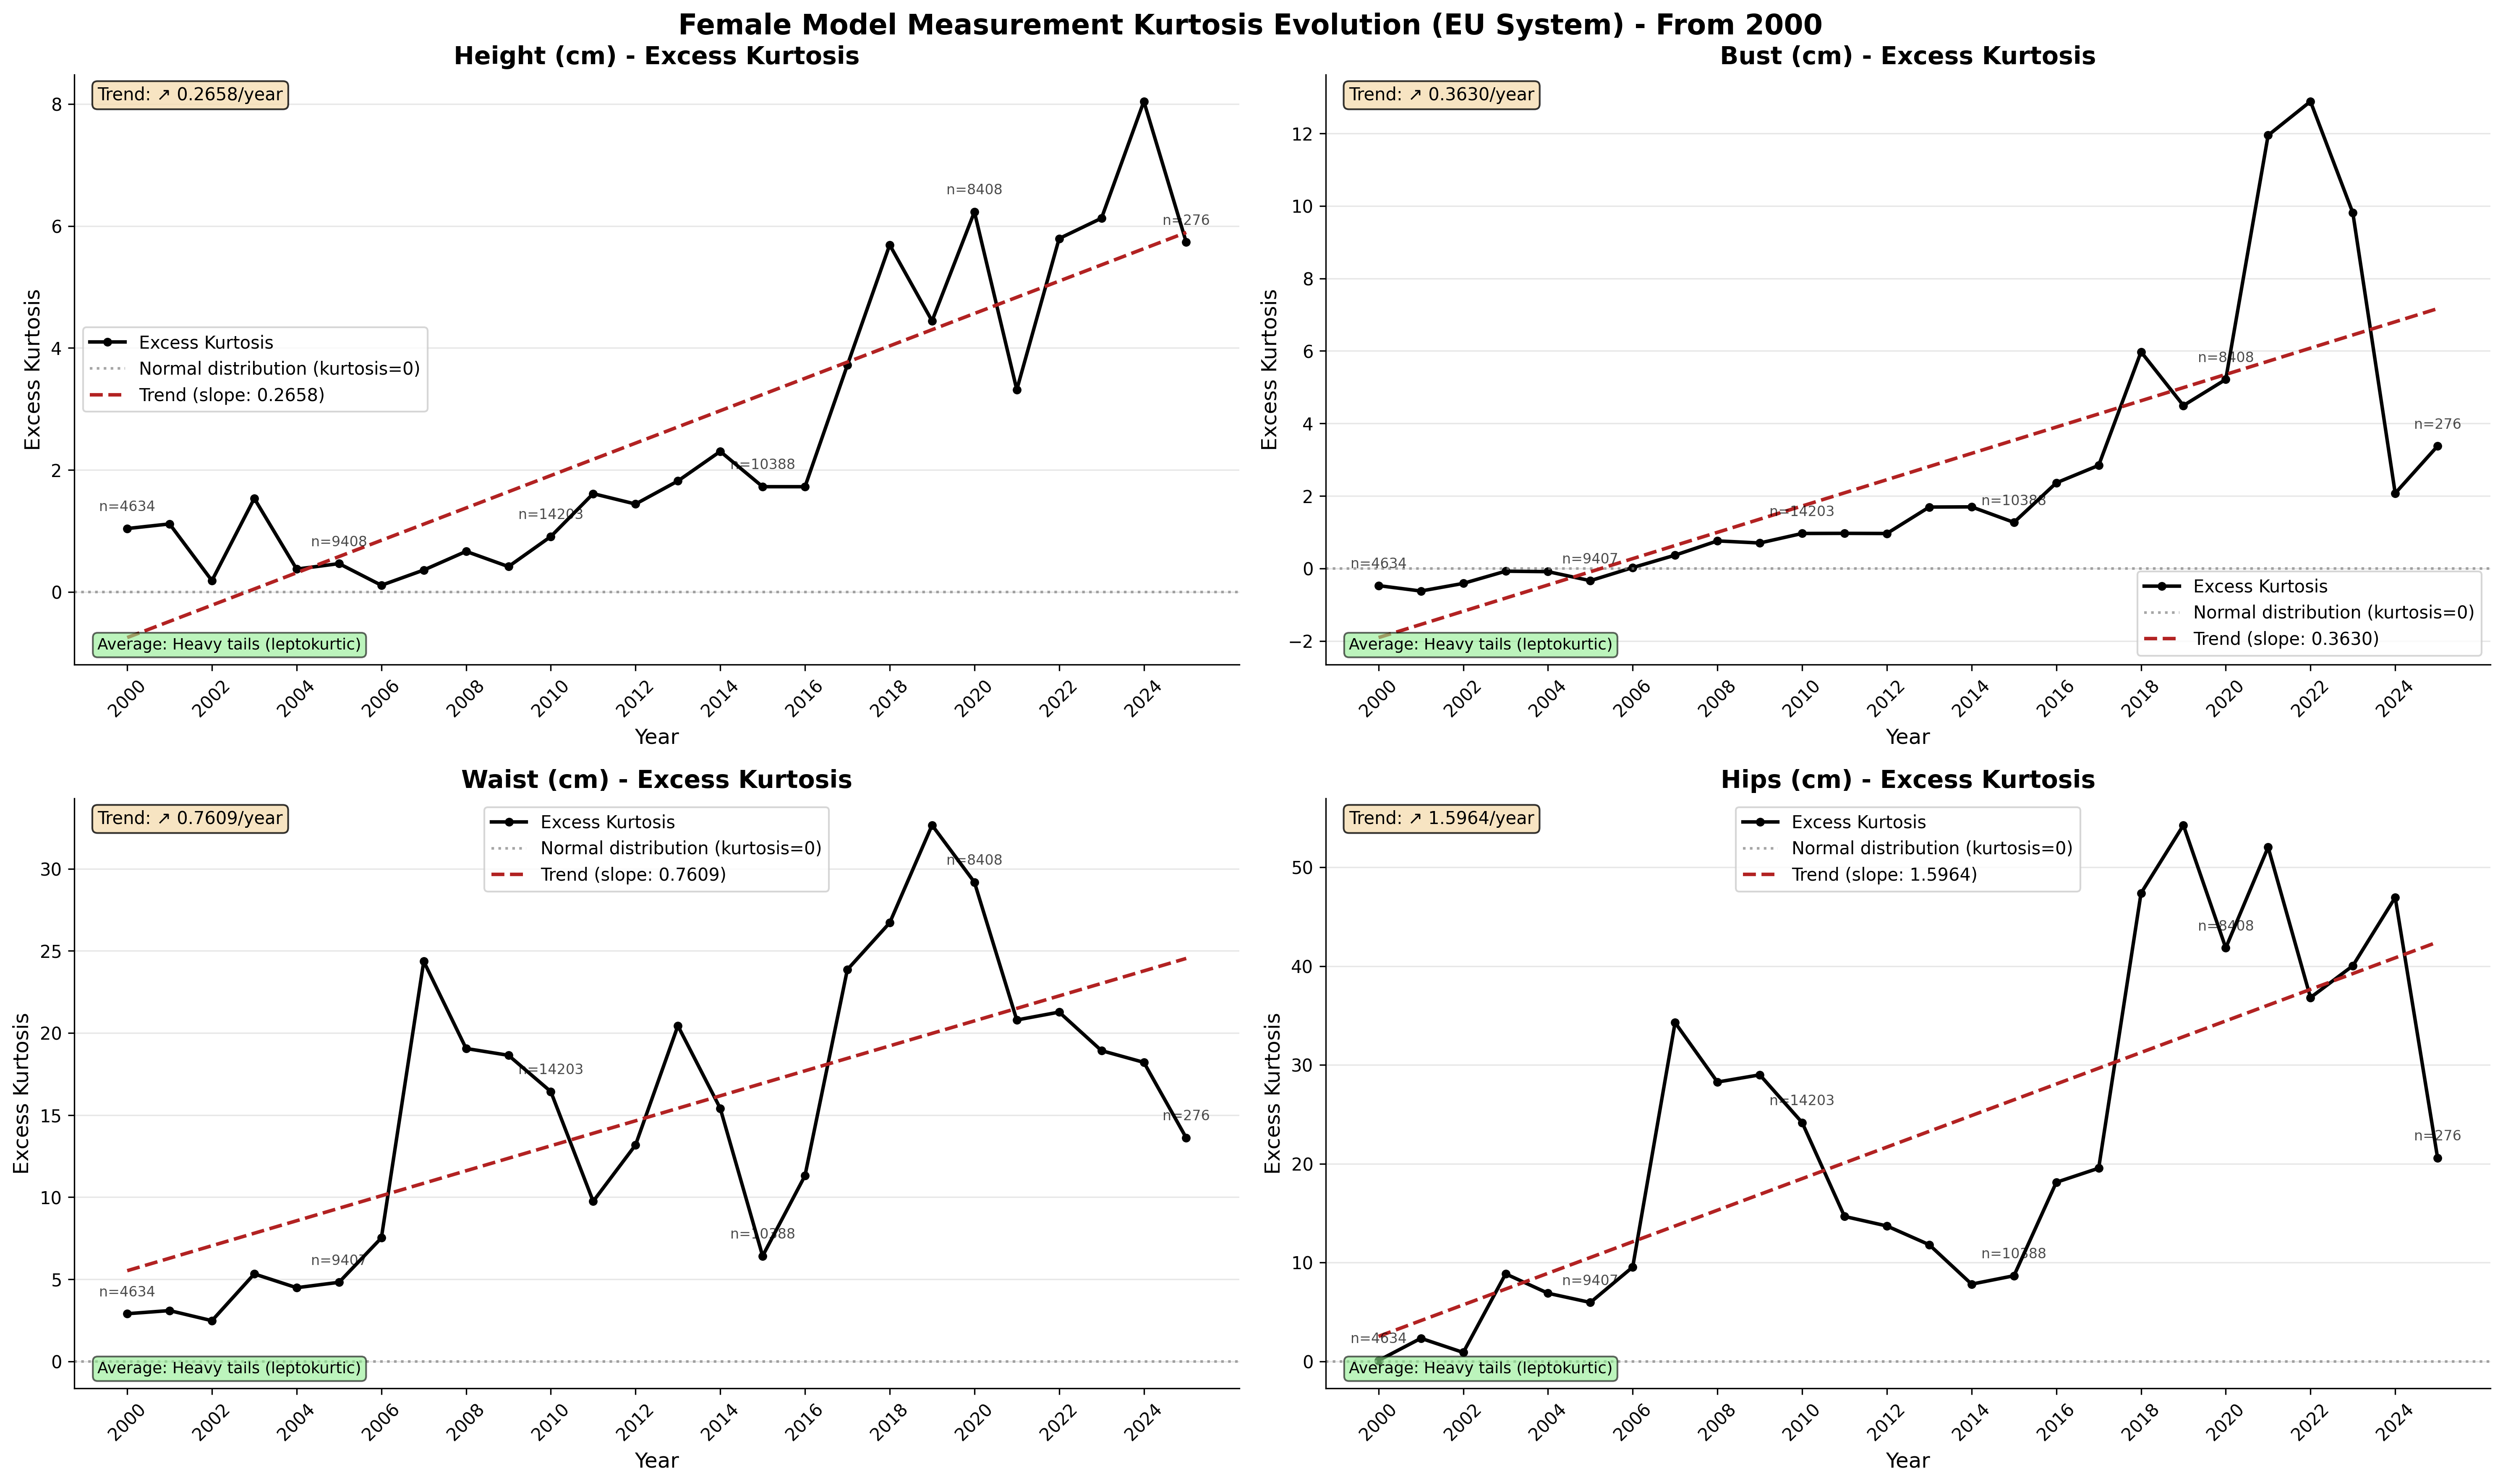
\includegraphics[width=\textwidth]{figures/kurtosis_evolution_female_eu_from_2000.png}
                \end{figure}
            
        
        \end{columns}
\end{frame}


\begin{frame}
    \Large{
        \begin{center}
            \textbf{How does it compare with general population?} \\
            \vspace{1em}
            Are these outliers truly outliers?\\
        \end{center}
    }
\end{frame}


%------------------------------------------------
\section{Comparison with General Population}
%------------------------------------------------

\begin{frame}[t]
    \frametitle{Comparison with General Population}
    \begin{columns}
        \column{0.65\textwidth}
            \begin{figure}
                    \begin{center}
                    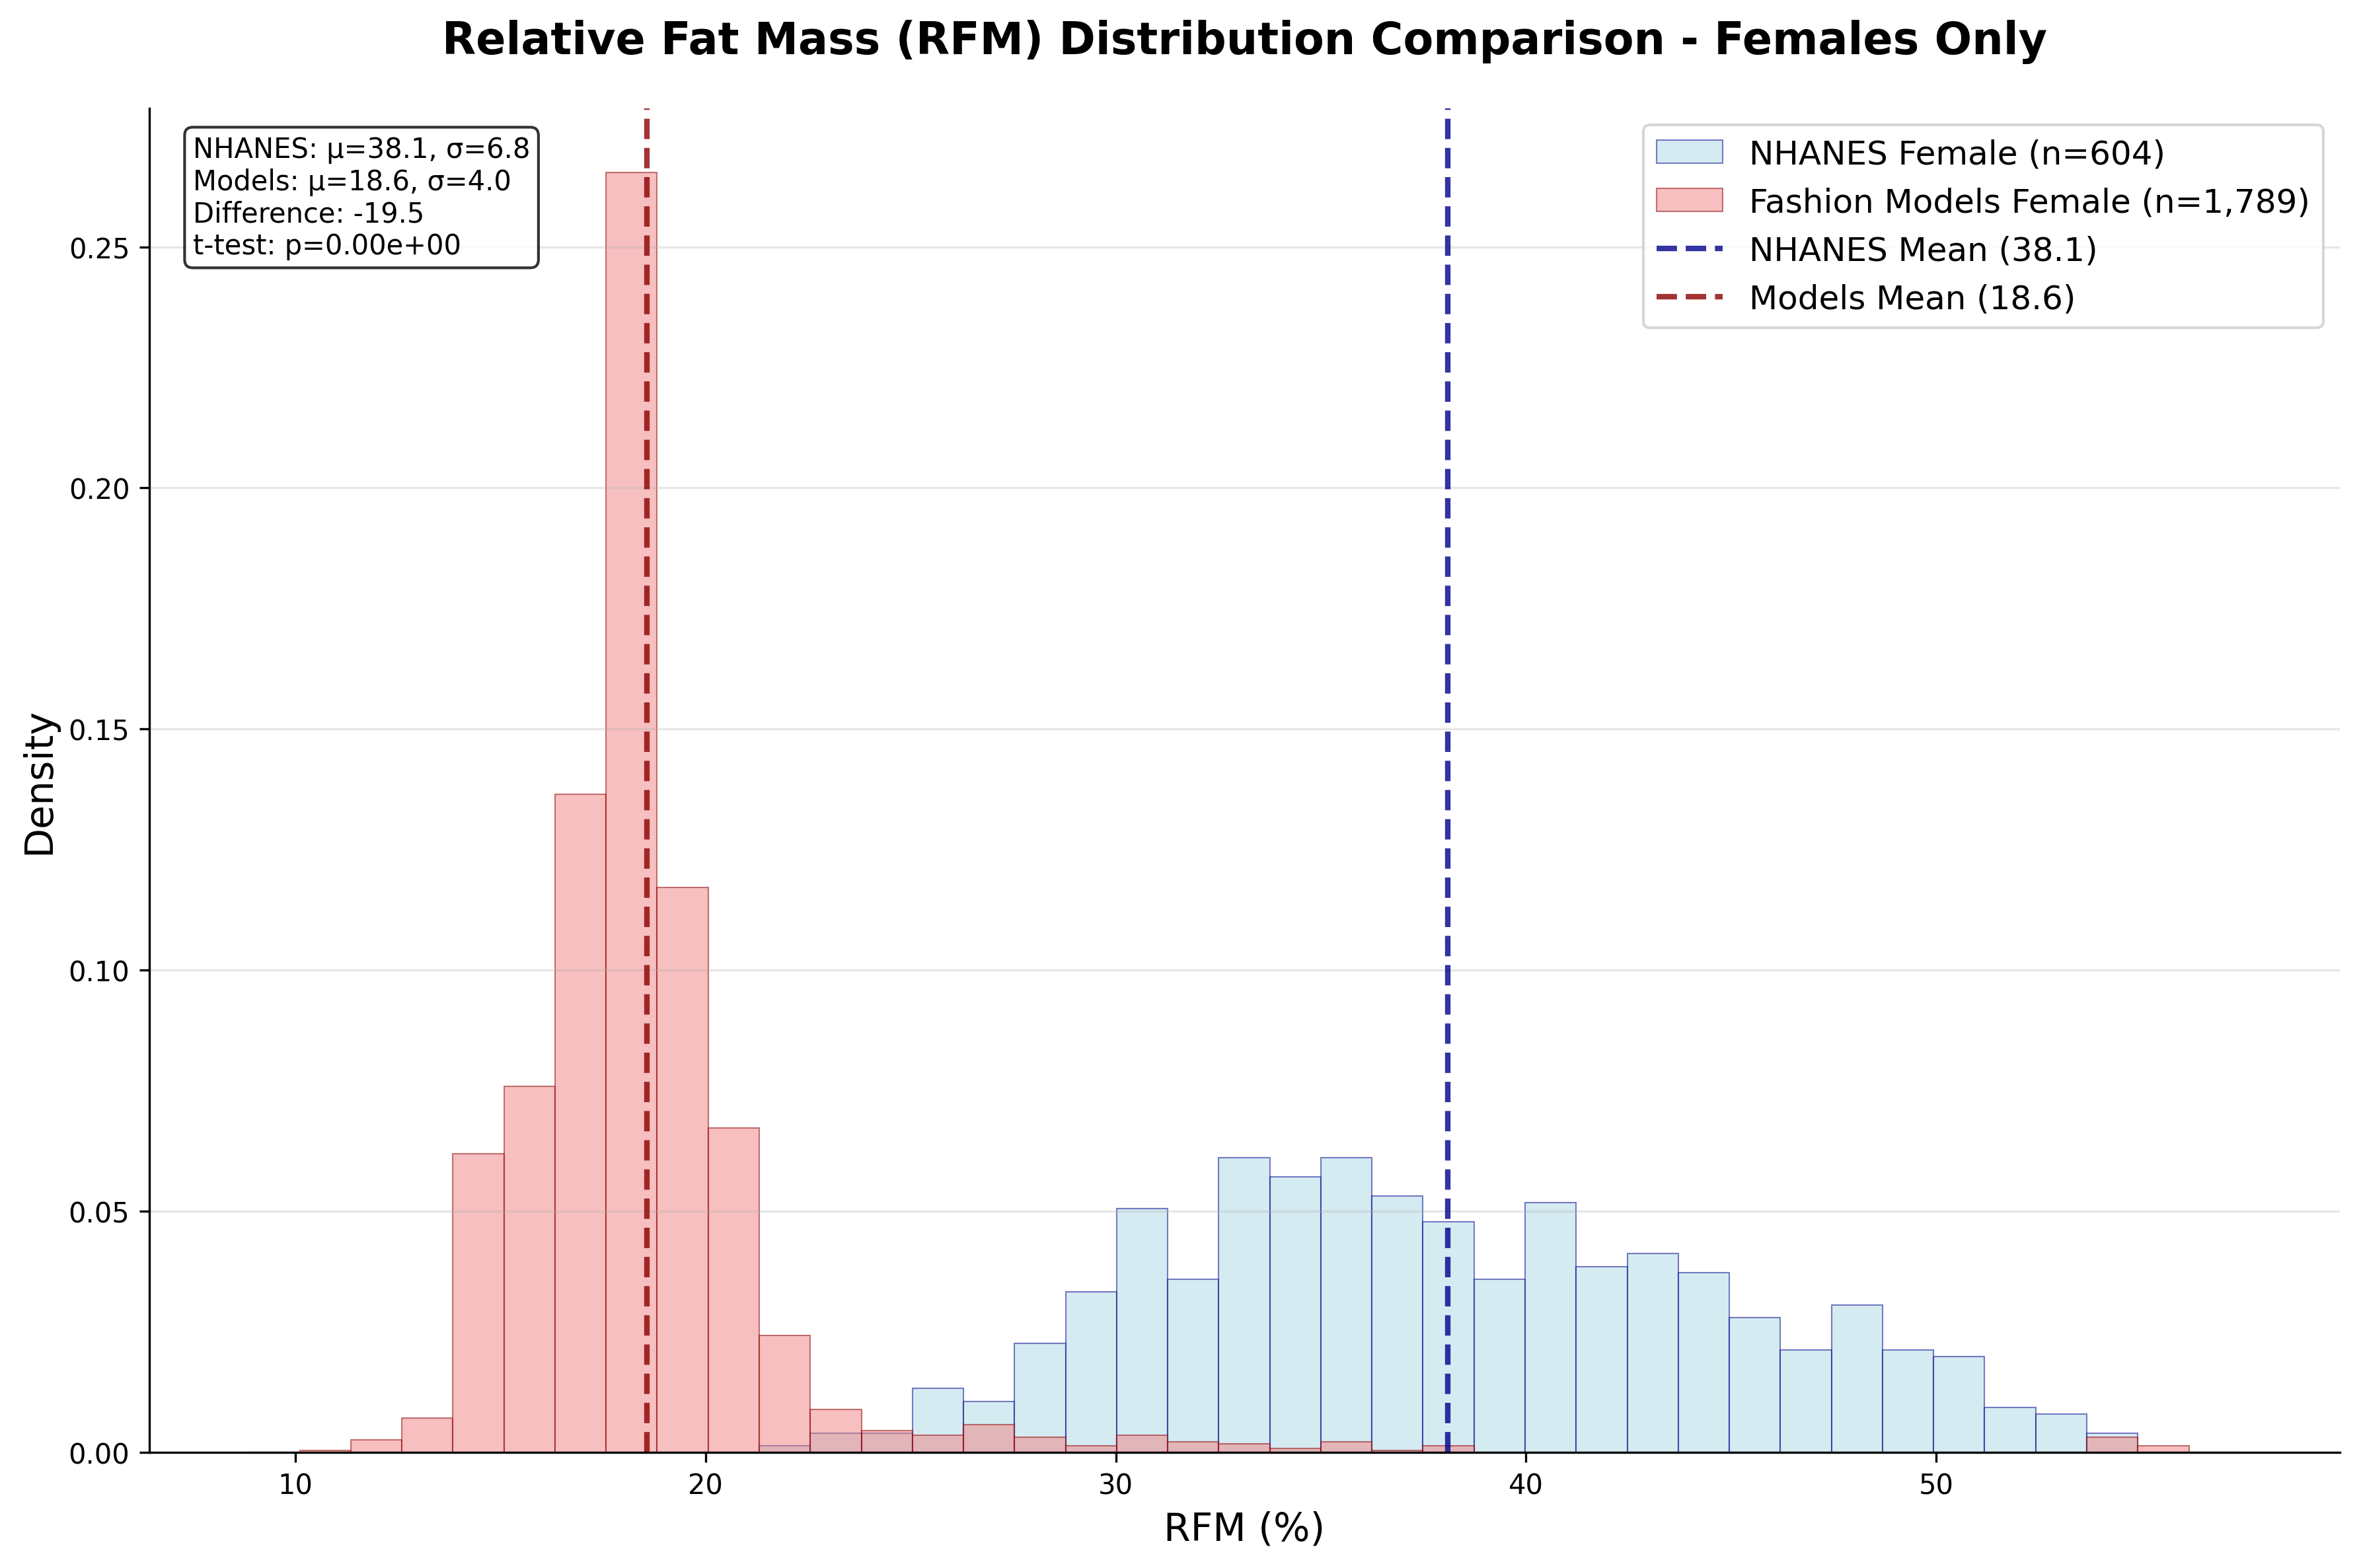
\includegraphics[width=\textwidth]{figures/rfm_female_distribution_comparison.png}
                    \end{center}
                \end{figure}

        \column{0.35\textwidth}
        \textbf{Relative Fat Mass (RFM)}: \\
            % \begin{equation}
            %     \text{RFM}_{\text{female}} = 76 - \left(20 \times \frac{\text{Height (cm)}}{\text{Waist Circumference (cm)}}\right)
            % \end{equation}
            RFM is a measure of body fat based on height and waist circumference
            \begin{itemize}
                \setlength{\itemsep}{0.6em}
                \pause \item Fashion models show lower RFM than general population
                \pause \item Models' RFM distribution is more concentrated around lower values
            \end{itemize}
    
    \end{columns}

\end{frame}

\begin{frame}{Conclusion Body Measurements}
    \begin{itemize}
        \setlength{\itemsep}{0.8em}
        \pause \item Body measurements show increasing diversity, but driven by outliers
        \pause \item Models' body measurements differ significantly from general population
        \pause \item Fashion modeling reflects a specific subset of beauty standards, not the general population
    \end{itemize}
    \pause
    \vspace{1em}
    \begin{block}{Key Insight}
        Fashion modeling increasingly includes diverse body types, but still represents a very narrow segment of population.
    \end{block}
    
\end{frame}
%------------------------------------------------
\section{Intersectionality of Diversity}
%------------------------------------------------


\begin{frame}
    \Large{
        \begin{center}
            We showed that body measurements and ethnic diversity in fashion modeling have increased over the past two decades.\\
            %Are these two evolution linked?
                        \vspace{1em}

            \textbf{How do these two evolutions relate?}\\
        \end{center}
    }
\end{frame}


\begin{frame}[t]
    \frametitle{Intersectionality of Diversity}
    \begin{figure}
            \begin{center}
            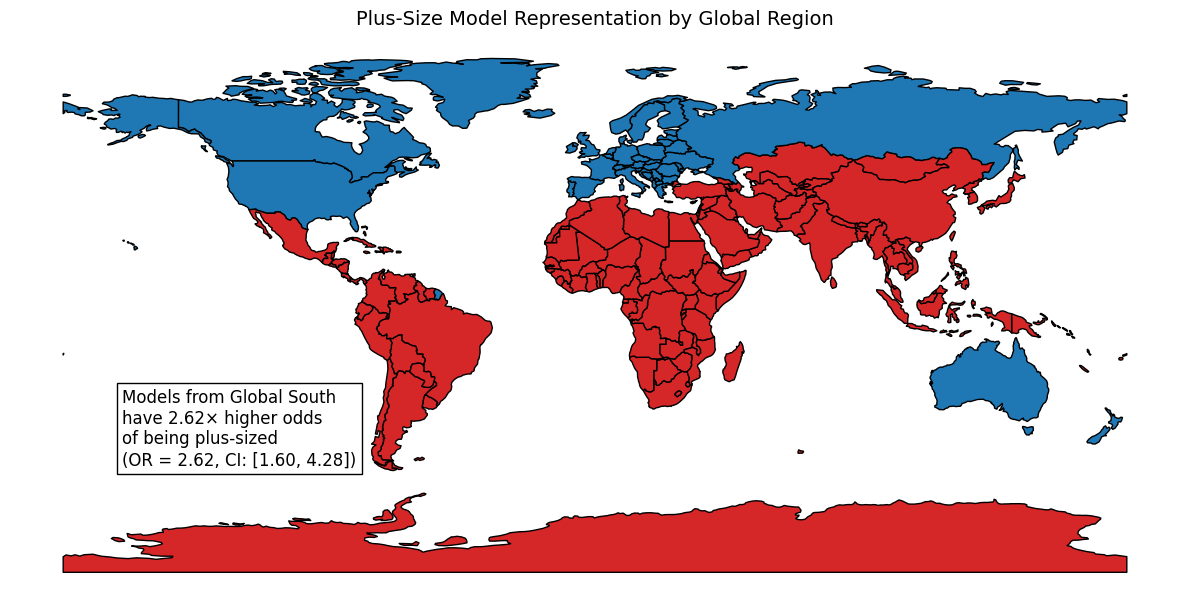
\includegraphics[width=0.9\textwidth]{figures/map_oddratio.png}
            \end{center}
        \end{figure}
\end{frame}

\begin{frame}[t]
    \frametitle{Evolution of Intersectionality of Diversity}
    \begin{figure}
            \begin{center}
            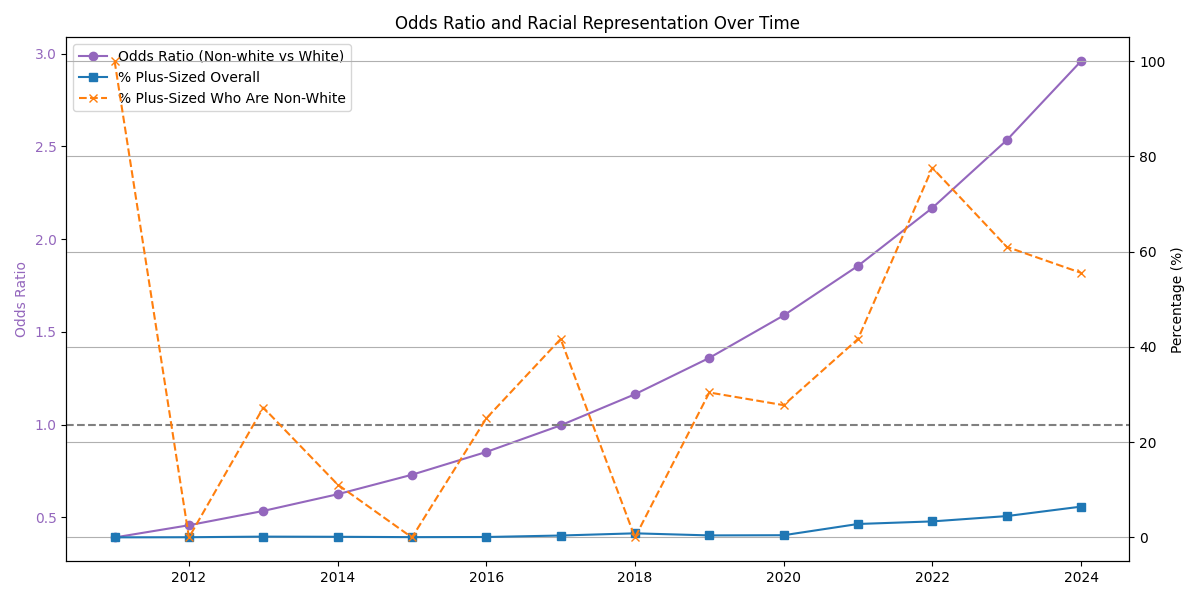
\includegraphics[width=0.9\textwidth]{figures/oddratio.png}
            \end{center}
        \end{figure}
\end{frame}

\begin{frame}[t]
    \frametitle{Breakdown Intersectionality of Diversity}
    \begin{figure}
            \begin{center}
            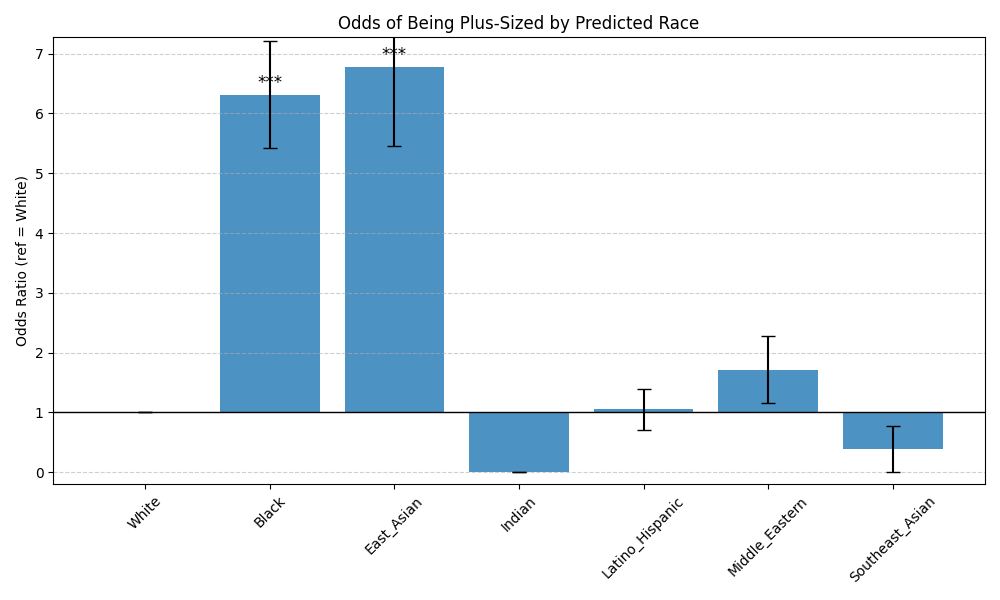
\includegraphics[width=0.8\textwidth]{figures/oddratio_race.png}
            \end{center}
        \end{figure}
\end{frame}

%------------------------------------------------
\section{Conclusion}
%------------------------------------------------

\begin{frame}{Conclusion}
   \pause \begin{exampleblock}{Research Question}
        How have beauty standards in fashion modeling evolved over the past two decades, and what does this reveal about broader cultural shifts in human representation?
    \end{exampleblock}
    \pause
    \begin{block}{Conclusion}
        \begin{itemize}{\setlength{\itemsep}{1em}}
            \pause \item Fashion runway can be used as a lens for studying shifting societal standards of beauty and representation
            \pause \item There is a clear trend toward greater diversity in fashion modeling (body measurements, visual traits, and ethnic diversity)
            \pause \item However, this diversity is still driven by outliers
            \pause \item And it does not reflect the general population
            \pause \item Intersectionality of diversity shows that ethnic diversity and body measurements diversity are linked
        \end{itemize}
    \end{block}
\end{frame}

%------------------------------------------------

% \begin{frame}{References}

%     % \footnotesize
%     % \bibliography{../diversity_fashion/bibliography}
%     % \bibliographystyle{unsrt}
% \end{frame}

%------------------------------------------------

\begin{frame}
    \Huge{\centerline{\textbf{Thank You for Your Attention!}}}
    \vspace{1em}
    \Large{\centerline{Questions \& Discussion}}
    \vspace{1em}
    %website
    \Large{\centerline{Website/Bluesky: \url{louisboucherie.com}}}
\end{frame}

%----------------------------------------------------------------------------------------

\end{document}